\documentclass{beamer}
\usepackage{pgfpages}
\usepackage{amsmath}
\usepackage{amsfonts}
\usepackage{fontspec}
\usepackage{xunicode}
\usepackage{xltxtra}
\usepackage{color}

\usepackage{beamertheme_atilla/beamerthemeAtilla}

\defaultfontfeatures{Mapping=tex-text}
%\setromanfont{Linux Libertine O}
\setsansfont{FreeSans}

\setbeameroption{show notes}
\setbeameroption{show notes on second screen=left}

% Hack to allow XeTeX to produce wide pdf
\renewcommand\pgfsetupphysicalpagesizes{%
	\pdfpagewidth\pgfphysicalwidth\pdfpageheight\pgfphysicalheight%
}

% CUSTOM COLORS ===============================================================

\definecolor{gray}{rgb}{0.5,0.5,0.5}
\definecolor{darkgreen}{rgb}{0.0,0.5,0.0}
\definecolor{mygreen}{rgb}{0,0.6,0}
\definecolor{mygray}{rgb}{0.5,0.5,0.5}
\definecolor{mymauve}{rgb}{0.58,0,0.82}
\definecolor{myorange}{RGB}{246,177,50}

% CUSTOM COMMANDS =============================================================

\newcommand\fixme{\textrm{\textbf{\textcolor{red}{FIXME: }}}}
\newcommand\todo{\textrm{\textbf{\textcolor{myorange}{TODO: }}}}
\newcommand\click{{\Large \textrm{\textbf{\textcolor{red}{CLICK! }}}}}
\newcommand\mytilde{\raise.17ex\hbox{$\scriptstyle\sim$}}
\newcommand\okeanos{\raise.17ex\hbox{$\scriptstyle\sim$}okeanos }
\newcommand\spc{\hfill \\}
\newcommand\dspc{\spc\spc}

\AtBeginSection[]
{
	\begin{frame}
		\frametitle{Table of Contents}
		\tableofcontents[currentsection]
	\end{frame}
}

% PRESENTATION SETTING ========================================================

\author{Αλέξιος Πυργιώτης}
\title{Σχεδίαση και Υλοποίηση Μηχανισμού Κρυφής Μνήμης για
	Κατανεμημένο Σύστημα Αποθήκευσης σε Περιβάλλον
	Υπολογιστικού Νέφους}
\institute{Εθνικό Μετσόβιο Πολυτεχνείο}
\date{\today}


\begin{document}
\chapter{��������}
� ���������� ����� �������� ���� ���������� ��������� �����
�����������. ������, � ����������� ���������� ��� ����������� ���
�����, ����� ���������������� ���� ��� �������-������ ��� ���
����� ��������� ��� ��� ���������. ��� �� ����������� ������ �
��������� ���������� ��� �� ����� ��� ������ � ��������� ��� �
����������� ���, � ���������� ����� ����������� ��� �������������
����.

� �������������� �����, ����� ��� ������� ��� ��������� �����,
���� ���� ����� ������� ���� �������� ����� ���� ���������� ���
�����������, �������������� �� ���������� ������ ���������� ���
�������� \cite{Berners-Lee01}. ��� ������������ ����� ��
���������� ��������� ��������� �� ������ ���� ����� �����������,
����� ��� ��� ��������������� ���������� ��� �����������,
��������������� �������� ��� ��� ����������� ��� �����������
$``$������������$"$. � �������� ����� ��� ��������, ��� ������ ���
��� ��������� ��� ����� ����������� ��������� �� ����������
��������� �� ����� ��� ����� ��� ��� �������� ����������� ���
������������ ��� ������� ��������� ��� ��������� ����� ���
�������� ��� ��� ���� ��� ������ ��� �����������.

��� ��� �� ��� ������ ������ ��� ��� �������� ��� ��������������
����� ����� �� �� ������� �� ����������� �� ������������ ��������
 ������ ���������. �� ��� ������� ���������� ����
����� � �������������� ����� ���������� ��� �������� ��� ��������
������� ���������� ��������� ���� ����� �� ��������� ��������
������ \en{(Peer-to-Peer systems)}.

��� ������� �������� ������ ����������� ��� ��� ������ ���������
������������� ������, �� ������ ������������� �� ����� ���
��������� ���������. �� ��������� �������� ������ ���
���������������� ������ ������ ������ ��� ��� ��������� �������
��������, ����� ���� ������ ����������� ����������� ���������. �
��������� ����������� ��� ����������� ��� ���� ������� �� �����
������ �������� \en{(keyword-based search)}.

� ������ ��� ��� ����������� �����������, �� ��������� �� ���
�������� ��� �������������� �����, ������� ��� ��������� ��������
������ ��� ����� ��������� �� ������� \en{(schema-based
peer-to-peer systems)}. ��� ��������� ���� ���� ������
������������ ��� ����� �� ���� �� ����� ��������� �� ������
��������� ��������. �� ����������� ��� �������������� ����� ������
�� ���������� ��������� ��� ��������� ���� �������� ��� ��
�����������.

�� ������� \en{RDF} ����� ��� ������ �������� �������������
�������������. �� ��� \en{RDF} ������ ��������� �������� ���
����������� ��� ����� ���� �������, ����������, ����������� �.�.�.
��� �������� ��� �������� \en{RDF} ����� �� \en{RDF Schema} ��
����� ������� ����������� ���������� �������� ������������ ���
����� ����� ��� ��� ������� ������ ����. �� \en{RDF Schema}
��������� �� ������� ��� ��������� ������� ������� ��� �� ���� ���
������������������ ����������. � ������ ������� ����� ��� ���
������� \en{RDF} �� ��������� ��������� ���������� ��� ���
�������.

��������������� ������ ��� ����������� ��� �������������� �����
�������� �� �������������� ��������� �������� ������ �� ��������
������������������ �� ����� �� ������������ ������ ���� ����������
�� ����� ��� �� ����� �� ���������� ���������� ��������� ���
����������� ��� ����� ��� ���������� �� ������ �������.


\section{����������� ��� ������������}
�� ������ ������ ��� ��������� ��� �� ��������� �������� ������
��� ����� ��������� �� �������, ����� ��� �� ������� �� ������ ��
��������� ��� �� ������������ ��������, ����������� ��� ���������
����. ��� ������������ ����� �������� ���� ������������:
\begin{enumerate}
\item � ����� ���������� ������� �� ������� ��� �������� ����� ��
����� �� ������������� ���� �� ������ \cite{KokkinidisC04}. ��
��������� ������������� ��� ������������ �� ���� �� ���� �����.
��� ������ ���� �� ���� ���� ��� ������������ �� ����������� ����,
���� ��� ���������� �� ������ ������ ���� ����������. ���� �� ���
������� ���������� ���� ����� � ���������� ����� ���������� ���
��� �������� ������� ��� �� ��������� ��� ����� ������ ��������.
\item � ������� ���������� ����� ��� ��������� �� ���� ����� �� �������� ����� ����� �����.
�� ��������� ������������� �� ���� ��� ����� ��� ������������ ��
���� ���� �������, ���� ���� ����������� ��������������� ���������
\en{(query reformulation)}. � ���������� ���� ������� ��� ������
������� ������������� \en{(mapping rules)} \cite{Piazza}. ����, ��
��� ������� �������� ������ �� ������ ������� �� �������� ��� ��
�������� ��� ������ �������. ��� ����� ������ �������� �� ���
�������� �� �������� ��� ������ ������ ��� ������ ������ ��
�������� ������� �������������. ������, �� ������� �����
���������� ������������ ��� ����� ������� � ��������� ����.
\end{enumerate}

����������� ��� ������������ ����� � �������� ���� ����������
�������� ������ ��������� �� ������� �� ����� (�) �� ��������� ���
������� �������� ���� ����� ��� �������� ��� (�) �� ����� ���
���������� ��������������� ��������� ����� ��� ������ ����������
������� ������������� ������ ��������. �� ������� ������ ���������
������� ��� ��� ������� ��� ������������ ��������, ��� �������
��������� ��� ����� �� ���������� ��������� ���������������
���������. ������������ ������� �� ������� \en{RDFS} ��� ���������
���������-����� \en{(views)} ���� ������� �������� (��������
�����).

��� ���������� ��������� ��� ���������� ����� �� ���� � ���������
�������������� ��������� ������ ��� ���������. ���� ��������� ��
���������� �� ���� �� ������� �������� ������ �� ��� ���� ���
\en{RDF} ����� ������� �� �� ����� �� �������� ��� ������������
��� ��� ���������� �� �������� �� ���������� ������� �������� ���
������ �������. �' ��� ������ ������� �� ��������� �� �����������
�� ������ ����� ��� ����������� ��������� ��� ���������� � ���
��������.

\section{�������� ��� �����}
� ������� ���� ����� ���������� �� ���� ��������: ��� �������� 2
������� �� ��������� �������� ��� ������� ����������� ���
����������� �� �� ����������� ����. ������ ������������� �� ������
�������� ������, ��� �������� �� ������� \en{RDF} ��� �����
������� ��� ������ ��� ������� ��������� ��� \en{RDF}. ���
�������� 3 ������ ������������� �� �������� �� �� ���� ��������
��� ��� �������� ������� � ������ ��� ������������� ��������. ���
�������� 4 ������������� � ������� ��� � �������� ��� ����������,
������ � ��������� ��� ������������� ��� ��� ��������� ���. �
��������� ��� ���������� ��� ����������, �� ������� ��� �������
���������� ����� ��� ������������ ������� �� ��� ���������� ��� ��
���������������� �������� ��� ���������������� ������� ���
�������� 5. ��� �������� 6 ������������� � ������� �����
����������� ��� ���������� �� ���� ��� ������������ �������
������. ����� ��� �������� 7 ������� � ���������� ����� ���
������������ ��������, ����� ��� ����������� ����������.

\section{VM Volume storage}

\begin{frame}[t]{Intro}

	\note[item]{Σε μεγάλες εγκαταστάσεις, ξεφεύγουμε από το κλασσικό 
		μοντέλο του PC μας (το μηχάνημα έχει το σκληρό του δίσκο).  
		Συγκεκριμένα σε μια cloud υποδομή έχουμε:}
	\note[item]{\click}
	\note[item]{To VM που τρέχει σε φυσικούς κόμβους}
	\note[item]{\click}
	\note[item]{τον εικονικό σκληρό του δίσκo, το κλασσικό /dev/sda/}
	\note[item]{\click}
	\note[item]{Και τους storage servers}
	\note[item]{\click}
	\note[item]{Το ερώτημα είναι λοιπόν, πως το VM θα αποθηκεύει τα δεδομένα 
		του; Παράλληλα, τι γίνεται στην περίπτωση που θέλουμε *και* τα εξής;}
	\note[item]{\click}
	\note[item]{Εξήγησε τους όρους}

	\pause
	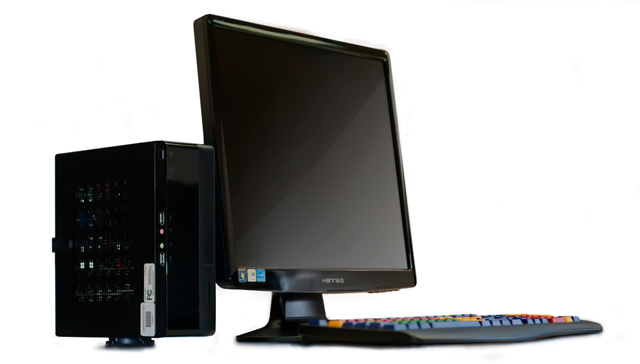
\includegraphics[width=.2\textwidth]{images/vm.jpg}\pause {\Huge +} 
	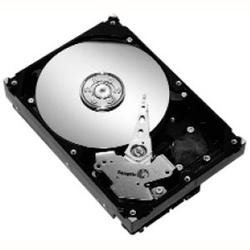
\includegraphics[width=.1\textwidth]{images/hdd.jpg}
	\pause
		 
\includegraphics[width=.05\textwidth]{images/link.png}
		 
\includegraphics[width=.15\textwidth]{images/cloud-server1.jpg}

	\pause\dspc
	\begin{itemize}
		\item Policy enforcement?
		\item Storage agnosticity?
	\end{itemize}

	\note[item]{Δηλαδή εφαρμογή δικών μας πολιτικών, χρήση οποιουδήποτε τύπου 
		storage}
\end{frame}

\begin{frame}{Our solution}

	{\Large Archipelago (many nodes)}

	\centering\makebox[\textwidth]{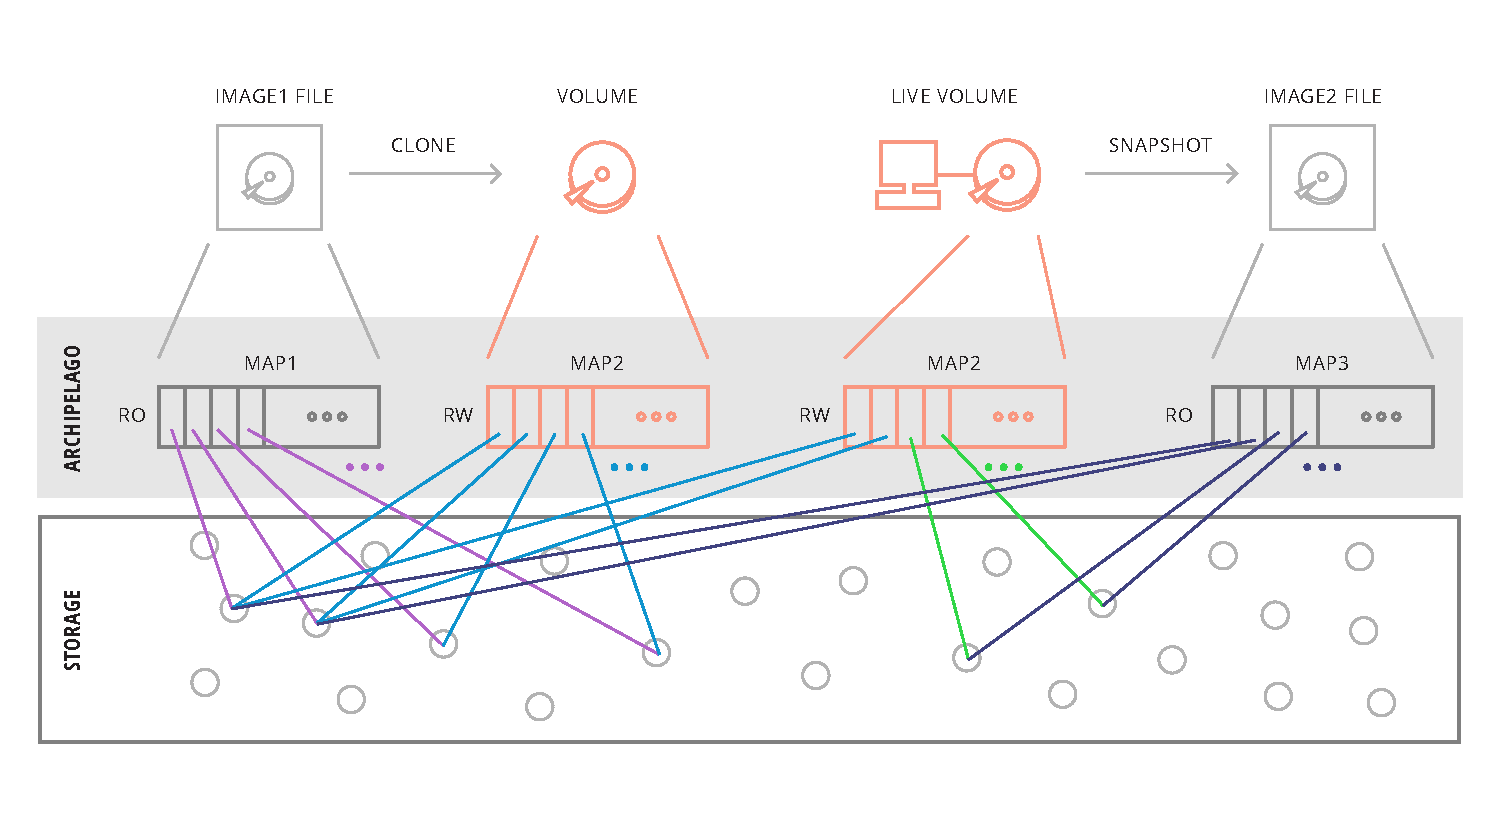
\includegraphics[width=0.8\textwidth]{images/archipelago-composition.pdf}}

	\spc

	Key features:
		1) Software-defined
		2) Distributed
		3) Modular
		4) Copy-On-Write
		5) Storage agnostic

	\note{Η λύση που χρησιμοποιήσαμε είναι το Archipelago}
	\note[item]{Πιο συγκεκριμένα, το Αρχιπέλαγο τρέχει στον host κόμβο. Είναι 
		ΑΚRIBΩΣ κάτω από τον σκληρό δίσκο του VM, το /dev/vda1. Τα δεδομένα 
		είναι στο storage}
	\note[item]{
		\begin{itemize}
			\item Software-defined: με το software ΟΡΙΖΕΙΣ το storage (εφαρμογή 
				policy, χρήση διαφορετικού storage για κάθε volume)
			\item τρέχει σε πολλούς κόμβους
			\item αποτελείται από διακριτά κομμάτια
			\item χρησιμοποιεί Copy-on-Write policy. NA αναφέρουμε εδώ ότι το 
				copy on write είναι μια πολιτική αντιγραφής ενός αντικειμένου.  
				To αντικείμενο σπάει σε κομμάτια τα οποία αντιγράφονται ΜΟΝΟ 
				όταν πάει να γράψει σε κάποιο από αυτά.
			\item μπορούμε χρησιμοποιήσουμε ότι storage θέλουμε
		\end{itemize}
	}
\end{frame}

\begin{frame}{Archipelago Architecture (single node)}
	\begin{center}
		  \makebox[\textwidth]{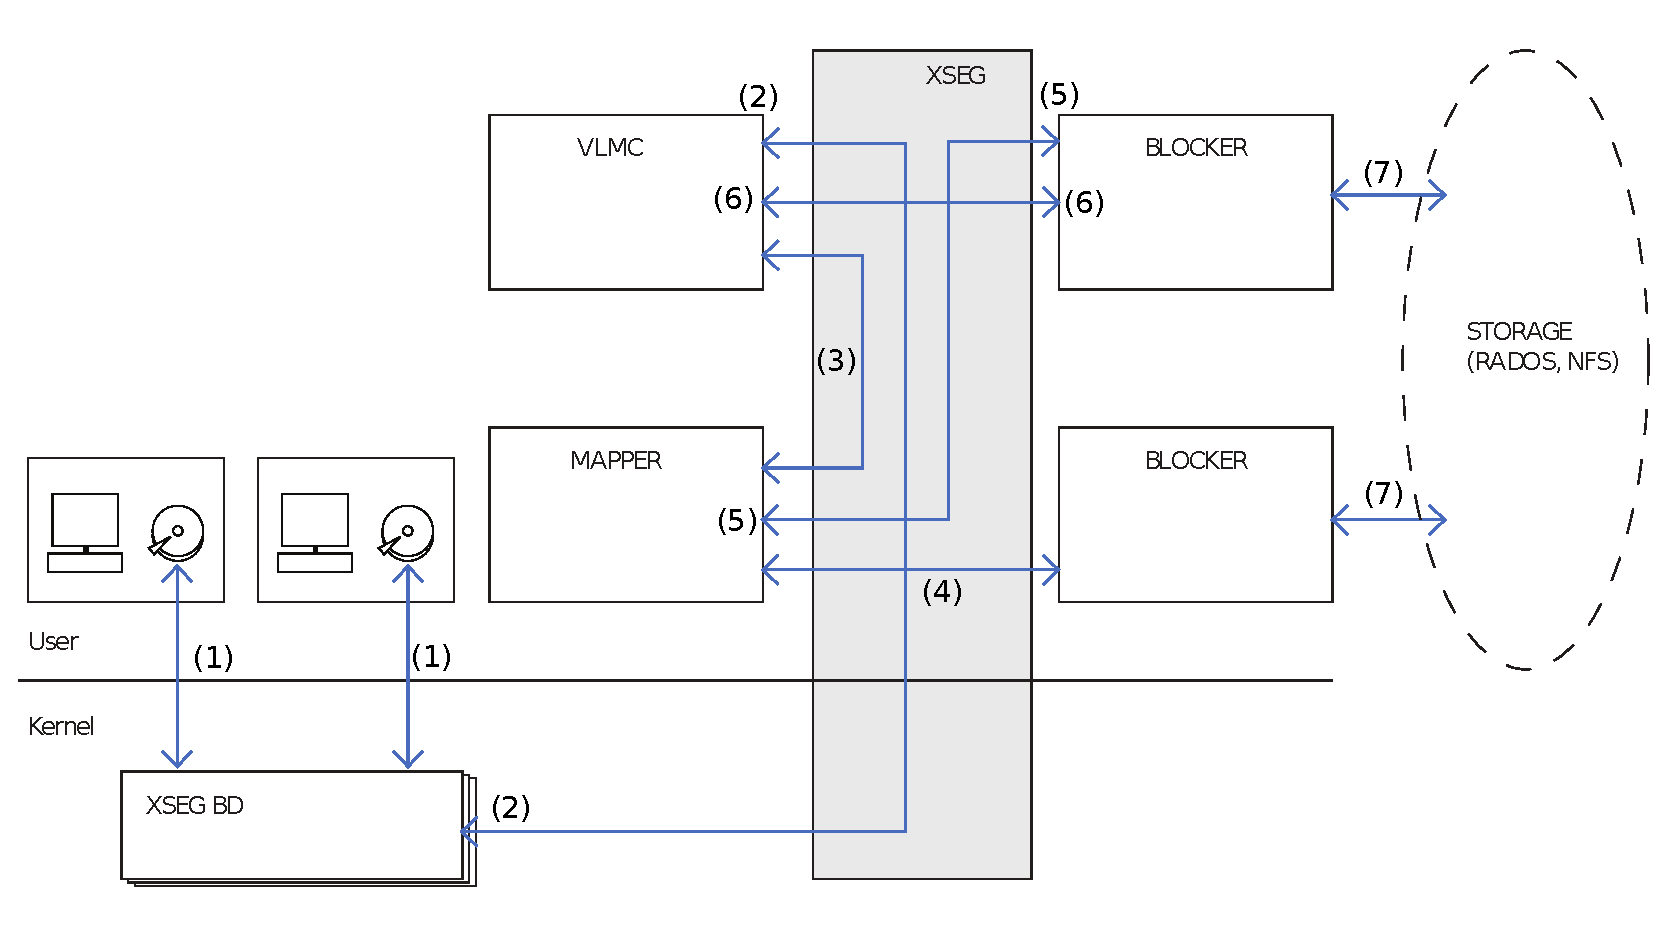
\includegraphics[width=0.9\paperwidth]{images/new_sxima_numbered.pdf}}
	\end{center}

	\note[item]{Βλέπουμε τώρα το Αρχιπέλαγο σε ένα κόμβο. Όλα είναι userspace 
		διεργασίες, μόνο ο xsegbd είναι kernel driver (όλα είναι PEERS)}
	\note[item]{Ας δουμε τη διαδρομή ενός IO request. To VM στέλνει αίτημα στο 
		δίσκο του. Ποιον δίσκο; /dev/vda1}
	\note[item]{ο δίσκος είναι εικονικός, θα το δει ο hypervisor (ο υπεύθυνος 
		για το virtualization του Virtual Machine) και θα το στείλει στον δίσκο 
		που το έχουμε πει.  (xsegbd)}
	\note[item]{Ο xsegbd είναι kernel driver και θα στέλνει τo αίτημα στο 
		userspace κομμάτι του Αρχιπελάγους το οποίο αποφαίνεται για τα 
		αντικείμενα τα οποία αντιστοιχούν στο αίτημα. Στο αίτημα αυτό θα 
		αναφέρεται ότι προέρχεται από το volume foo.}
	\note[item]{το παίρνει ο vlmc, ρωτάει τον mapper, από ποια αντικείμενα 
		αποτελείται; λέει ότι είναι το foo}
	\note[item]{μετά τα ζητάει από το storage μέσω των blockers. ΤΩΡΑ ΜΙΛΑΜΕ 
		για την έλλειψη στα δεξια}
\end{frame}

\begin{frame}{RADOS}

	The object store component of a promising technology
	\dspc
	Key features:
	\begin{itemize}
		\item Replication
		\item Fault tolerance
		\item Self-management
		\item Scalability
		\item Uses commodity hardware
	\end{itemize}

	\note{Αν και είμαστε storage agnostic, χρησιμοποιούμε ένα σημαντικό storage 
		backend, το RADOS. To rados είναι το object store component μιας πολλά 
		υποσχόμενης τεχνολογίας που μας δίνει τα εξής:
		\begin{itemize}
			\item Αντίγραφα ασφαλείας των δεδομένων
			\item Ανοχή στο χάσιμο αποθηκευτικών κόμβων
			\item Load balancing και αυτοδιαχείριση
			\item ειναι κλιμακώσιμο
			\item χρησιμοποιεί απλό hardware
		\end{itemize}
	}
	\note[itemize]{υ.γ. αντικείμενα είναι ονοματοδοτούμενη ποσότητα 
		πληροφορίας}
\end{frame}

\begin{frame}{Thesis motivation}
	\begin{itemize}
		\item RADOS has speed issues: Bandwidth < 7MB/s, Latency \mytilde10ms
		\item Request type: Block size: 4KB, parallel requests: 16
		\item Qualitative benchmark that depicts a hard workload
	\end{itemize}
	\spc
	Thesis goal: Mitigate RADOS speed issues.
	\dspc
	Observation:\\
	VM with page-cache of host enabled: Bandwidth > 90MB/s, Latency < 1ms
	\dspc
	Page-cache is great but it has many limitations:
	\begin{itemize}
		\item KVM and Linux kernel dependent (we REALLY want to avoid this)
		\item Unaware of CoW policies
		\item Difficult to manage
	\end{itemize}

	\note[item]{Αυτό το περίπλοκο σύστημα όμως δεν είναι αρκετά ταχύ.  Από 
		πραγματικές μετρήσεις σε ένα VM έχουμε ότι:...}
	\note[item]{Αυτά τα αποτελέσματα δεν είναι καλά}
	\note[item]{Στόχος διπλωματικής, απάλειψη του αντίκτυπου της επίδοσης του 
		RADOS στο Αρχιπέλαγο}
	\note[item]{Παρατηρήσαμε ότι αν ενεργοποιήσουμε την page cache έχουμε...}
	\note[item]{Η page-cache όμως έχει σοβαρούς περιορισμούς}
	\note[item]{Επίση, εμείς μπορεί να θέλουμε να cach-άρουμε σε ssd, να 
		κάνουμε replication, να έχουμε επιλεγόμενα επίπεδα αξιοπιστίας για κάθε 
		VM}
\end{frame}


\section{Caching}

\begin{frame}{Intro}

	Solution: Caching\\
	\spc
	Caching is:
	\begin{itemize}
		\item We have a slow medium
		\item Add a fast medium in a data path
		\item Transparently store the data that are intended for the 
			slower medium.
		\item Profit: later accesses to the same data are faster
	\end{itemize}
	\dspc
	Sounds familiar?

	\note[item]{Η κλασσική λύση σε τέτοια προβλήματα είναι η χρήση ενός 
		γρηγορότερου αποθηκευτικού μέσου για caching.}
	\note[item]{Για όσους δεν ξέρουν τι σημαίνει caching, θα το εξηγήσουμε 
		συνοπτικά: έχεις ροή δεδομένων, καταλήγουν σε αργό μέσο, βάζεις μπροστά 
		ένα μικρό αλλά γρήγορο μέσο, οι επόμενες προσβάσεις στη μνήμη θα είναι 
		πιο γρήγορες}
	\note[item]{Γιατί δε βάζεις μόνο γρήγορο, γιατί είναι ακριβά}
	\note[item]{Προφανώς αυτό το concept είναι γνωστό. Από που;}
\end{frame}

\begin{frame}
	\makebox[\textwidth]{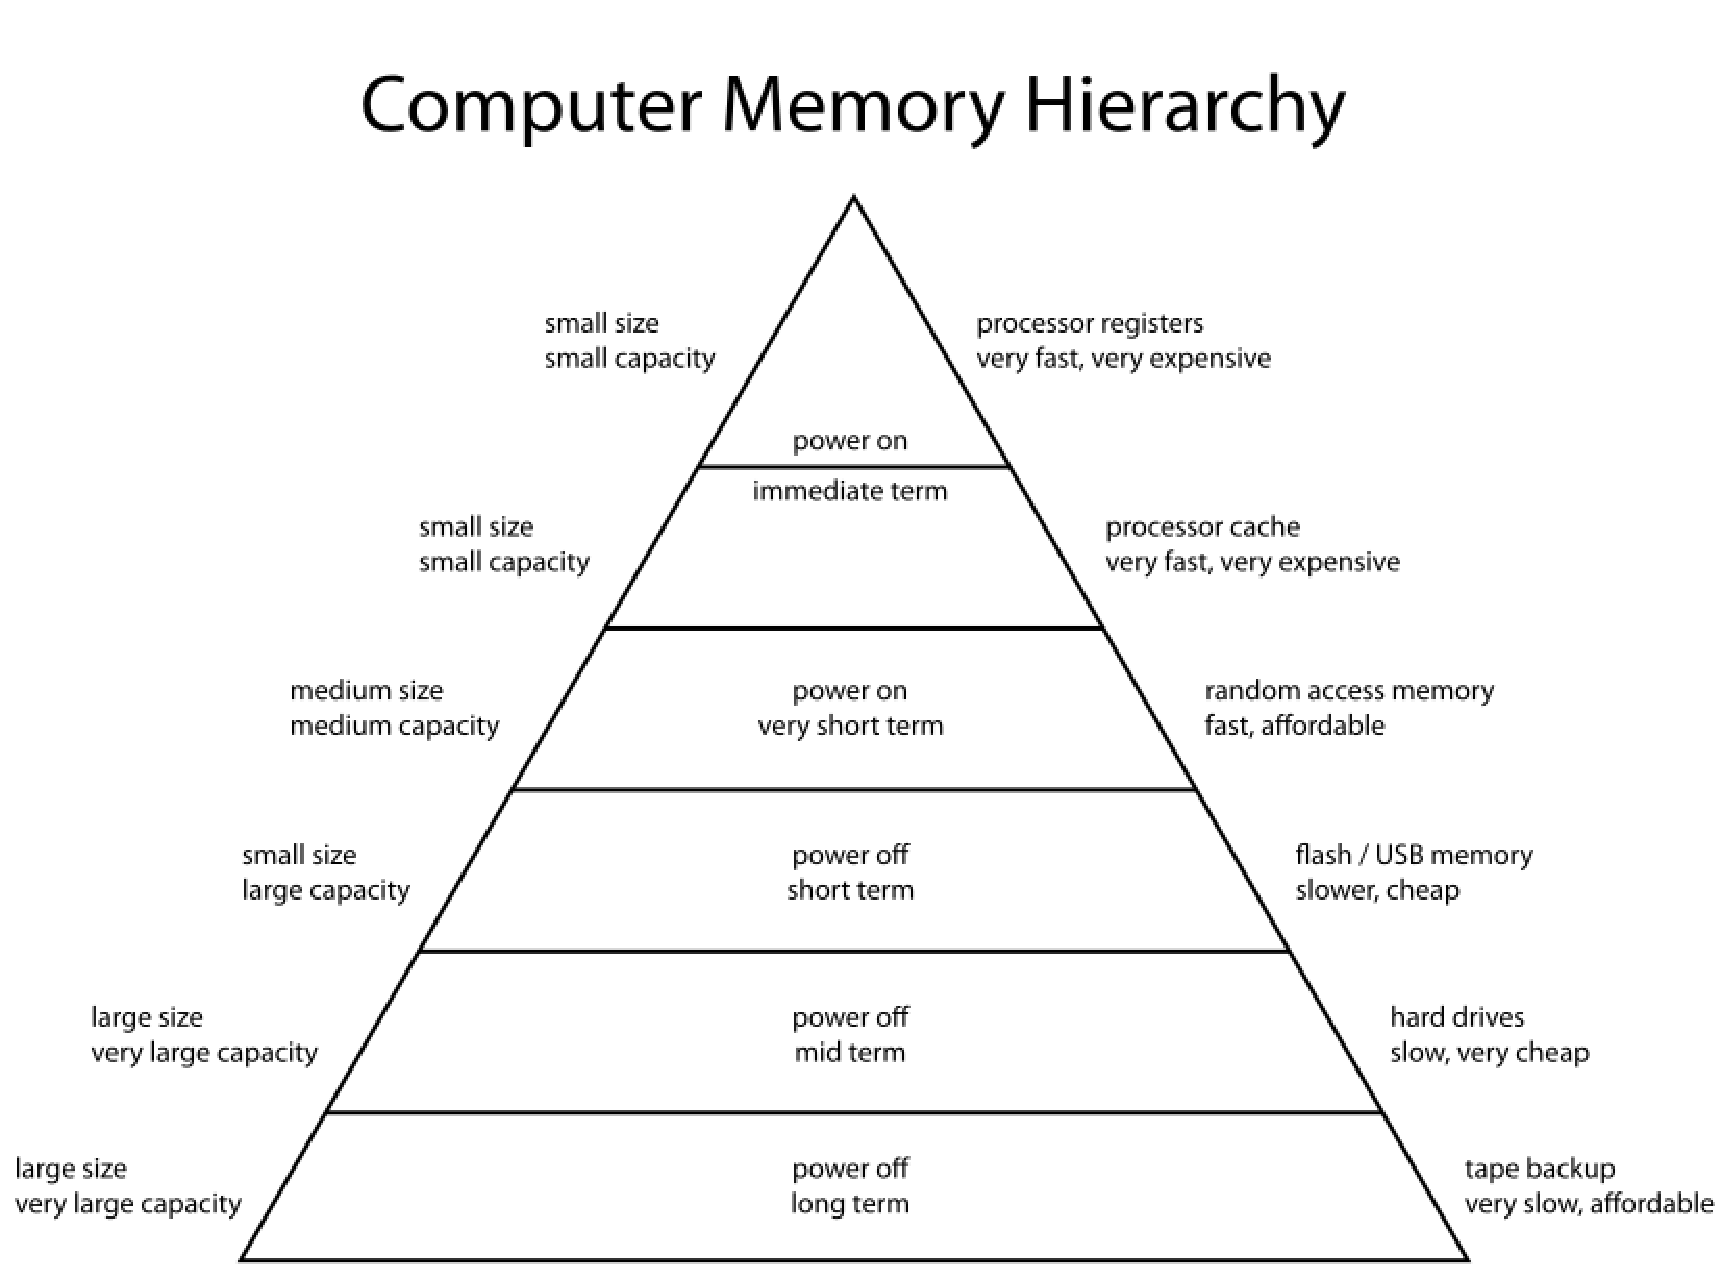
\includegraphics[width=0.8\textwidth]{images/mem-hier.pdf}}
	
	That's because every PC is built that way.

	\note[item]{Τρέχα}
\end{frame}

\begin{frame}
	Is there anything to help us?
	\dspc
	FACT: We are not the first to have speed issues\\
	Facebook, Twitter, Dropbox, every one has hit and surpassed their limits.
	\dspc
	There are solutions separated in two categories:
	\begin{itemize}
		\item Block-based caching
		\item Object-based caching
	\end{itemize}
	\note[item]{Τώρα που ξέρουμε τη λύση, υπάρχει κάτι που μπορούμε να 
		κάνουμε;}
	\note[item]{Υπάρχει κάτι έτοιμο; ΝΑΙ}
	\note[item]{Δυο κατηγορίες:
		\begin{itemize}
			\item βλέπουν τα δεδομένα σαν blocks ενός δίσκου
			\item βλέπουν τα δεδομένα σαν κομμάτια αντικειμένων
		\end{itemize}
		Διαφορά: \todo
	}
\end{frame}

\begin{frame}{Block-based caching solutions}

	Most notable examples:
	\begin{itemize}
		\item Bcache
		\item Flashcache
		\item EnhanceIO
	\end{itemize}
	\dspc
	Typically scale-up solutions.
	\dspc
	Pros: Simple, scale-up\\
	Cons: Unaware of CoW, kernel-space solutions, redundancy issues

	\note[item]{Δε θα επεκταθούμε γιατί έχουν κάποια βασικά κοινά:
		\begin{itemize}
			\item Kernel modules
			\item expose εικονικά block devices που δείχνουν σε 
				γρήγορα μέσα
			\item Καθαρά caching μηχανισμοί που παίζουν με writeback, 
				writethrough κτλ.
		\end{itemize}
	}
	\note[item]{Εξήγησε που μπαίνουν (xsegbd). ΠΗΓΑΙΝΕ στο archipelago}
	\note[item]{Παρότι είναι αρκετά απλοί, δε γνωρίζουν την CoW πολιτική 
		άρα χάνουν χώρο και είναι στον kernel (που δε θέλουμε)
	}
\end{frame}

\begin{frame}{Object-based caching solutions}
	Most notable examples:
	\begin{itemize}
		\item Memcached
		\item Couchbase
	\end{itemize}
	\dspc
	Typically scale-out solutions
	\dspc
	Pros: Distributed with no SPOF, can utilize unneeded RAM, user-space 
	solutions\\
	Cons: Memcached has no persistence, Couchbase cannot use RADOS as its 
	backend, more suitable for databases
	\note{Τα πράγματα γίνονται πιο ενδιαφέροντα εδώ:
		\begin{itemize}
			\item Κατανεμημένα συστήματα χωρίς ενιαίο σημείο αποτυχίας (SPOF), 
				μπορούν να τρέχουν εκτός host οπότε δεν το επιβαρύνουν, είναι 
				user-space λύσεις
			\item Memcached δε διατηρεί με ασφάλεια τα αντικείμενα που 
				cachάρει, couchbase δεν μπορεί να μιλήσει με RADOS 
		\end{itemize}
	}
\end{frame}

\begin{frame}{Conclusions}

	\begin{itemize}
		\item Most solutions far from Archipelago's logic
		\item Others not suited for storage and more suited for 
			databases
		\item Block-based caching might be good for the storage backend
		\item Must implement our own solution
	\end{itemize}

	\note{Οι λύσεις αυτές είναι μακριά από τη λογική και το I/O pipeline του 
		αρχιπελάγους. Είναι άσχετα συστήματα που πρέπει να επέμβουμε σε αυτά 
		για να κάνουμε αυτά που θέλουμε. Άρα πρέπει να κάνουμε τη δική μας 
		λύση}
\end{frame}
	

\section{Cached design}

\begin{frame}{Requirements}

	Design goals for cached:
	\begin{itemize}
		\item Create something close to the Archipelago logic
		\item Measure the best possible performance we can get
	\end{itemize}

	\note{Επιλέξαμε λοιπόν να δημιουργήσαμε τη δική μας λύση. Την ονομάσαμε 
		cached από το cache daemon}
	\note{Ορίσαμε τους εξής γενικούς στόχους:
		\begin{itemize}
			\item Να είναι κοντά στη λογική του Archipelago
			\item Η υλοποίηση να είναι όσο το δυνατόν πιο γρήγορη 
				για να δουμε αν μια Αρχιπελαγική λύση μας 
				βοηθάει
		\end{itemize}
	}
	\dspc
	Stricter requirements for cached:
	\begin{itemize}
		\item Nativity
		\item Pluggability
		\item In-memory
		\item Low indexing overhead
	\end{itemize}
	\note{Ακόμα, θέσαμε κάποιες πιο αυστηρές απαιτήσεις για την υλοποίηση 
		μας: 1)να είναι peer του Archipelago, 2) να μπορεί να ενεργοποιείται 
		και να απενεργοποιείται σε ένα σύστημα που είναι εν λειτουργία, 3)να 
		χρησιμοποιεί τη RAM, 4)ο indexing μηχανισμός να είναι γρήγορος}
\end{frame}

\begin{frame}{Cached design}
	\note{Εδώ βλέπουμε το design του cached. Ο cached μπαίνει ανάμεσα στον vlmc 
		και στον blocker και cach-άρει ότι άιτημα για αντικείμενα πάει στο 
		storage}
	\note{Οι εργασίες του cached χωρίζονται σε 5 κατηγορίες:}
	\note[item]{Στην διαχείριση των αιτημάτων από και προς vlmc, blocker}
	\note[item]{Στο indexing (εύρεση και καταχώρηση) των αντικειμένων}
	\note[item]{Στην υπο συνθήκες εκτέλεση εργασιών}
	\note[item]{Στην ασφαλή μετάδοση των cachαρισμένων δεδομένων στο 
		storage}
	\note[item]{Καθώς επίσης και στην ασφαλή επεξεργασία των cachαρισμένων 
		δεδομένων}
	\note[item]{\click}

	\begin{columns}[T]
		\begin{column}{0.65\textwidth}
			\includegraphics<1>[width=\columnwidth]{images/cached-design2.pdf}
			\includegraphics<2>[width=\columnwidth]{images/cached-design-comp2.pdf}
		\end{column}
		\begin{column}{0.35\textwidth}
			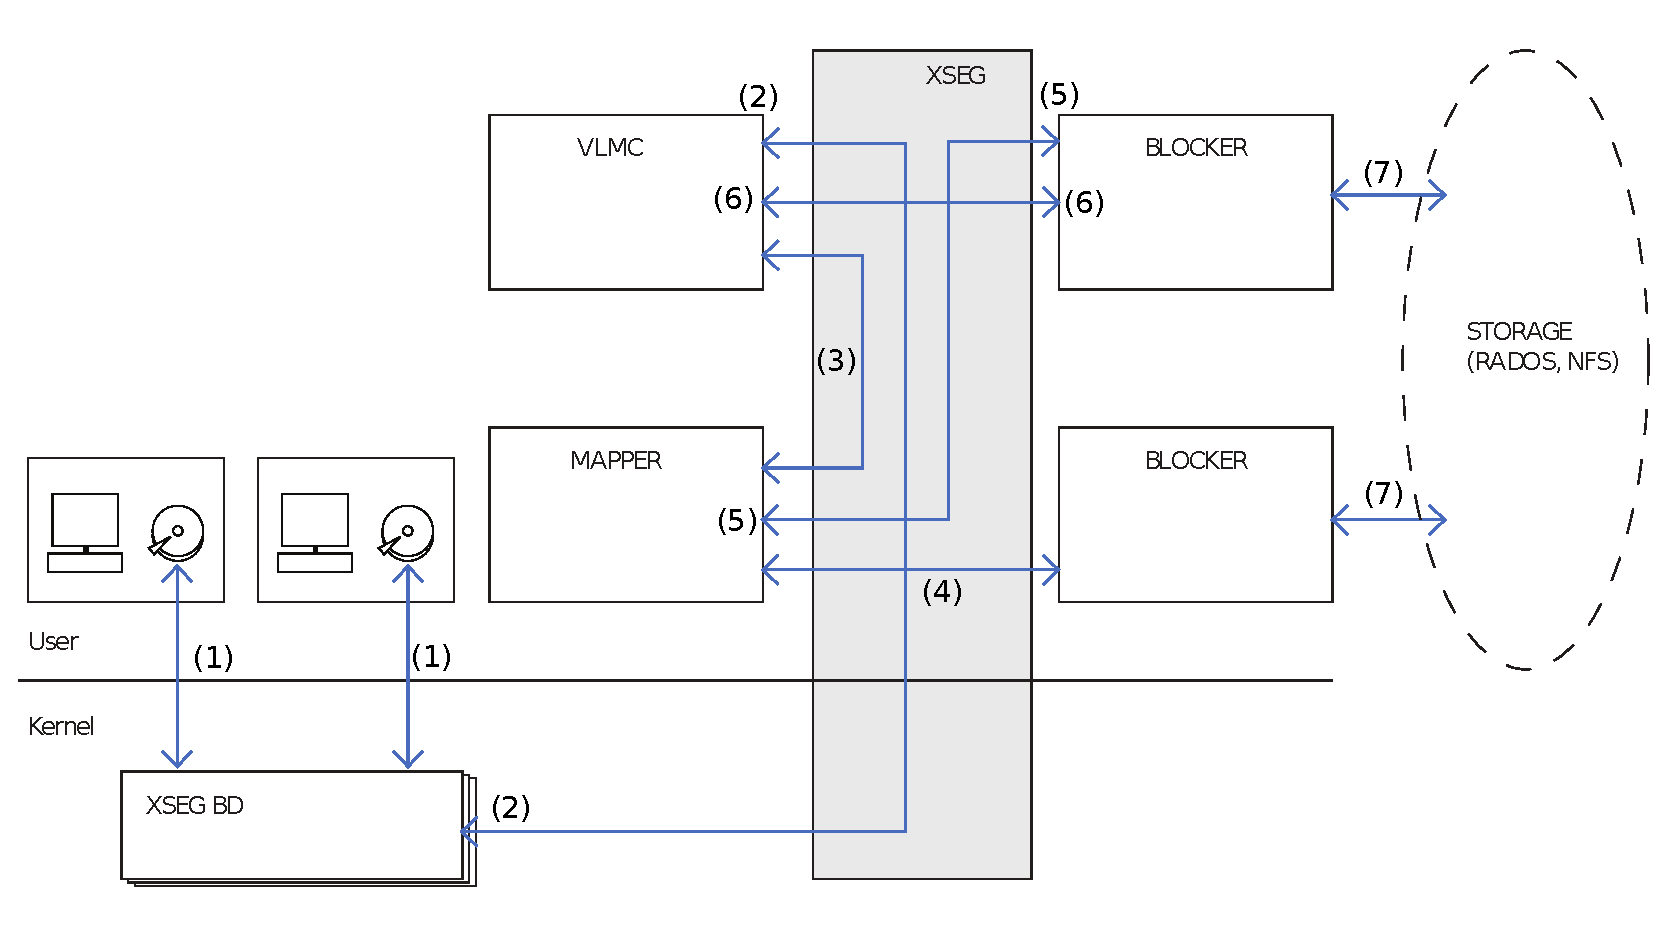
\includegraphics[width=\columnwidth]{images/new_sxima_numbered.pdf}
		\end{column}
	\end{columns}
	\note[item]{Και εδώ βλέπουμε τα διακριτά κομμάτια κώδικα που υλοιποιούν τα 
		παραπάνω και τα οποία θα συζητήσουμε ευθύς αμέσως}
\end{frame}

\begin{frame}{Xcache design}
	\centering\includegraphics<1>[height=0.6\textheight]{images/xcache-design.pdf}
	\centering\includegraphics<2>[width=\textwidth]{images/xcache-entry.pdf}

	Xcache is responsible for: 1) entry indexing, 2) entry eviction, 3) 
	concurrency control

	\note[item]{Αυτό είναι το xcache, που είναι υπεύθυνο για την
		\begin{itemize}
			\item Indexing των αντικειμένων
			\item Eviction αντικειμένων από την cache με τη χρήση LRU
			\item Χειρισμό προσβάσεων από πολλαπλά threads
		\end{itemize}
	}
	\note[item]{Έχουμε δυο hash table, το καθένα με το δικό του lock, ένα χώρο 
		που αποθηκεύονται οι εγγραφές των αντικειμένων και μόνο (όχι τα 
		δεδομένα, προσοχή) και μια στοίβα όπου κρατιούνται indexes των 
		ελεύθερων entries, προστατευόμενη από ένα lock.}
	\note[item]{To ένα hash table <αυτό> που κρατάει τα ονόματα των cached 
		αντικειμένων.}
	\note[item]{To άλλο hash table κρατάει τα ονόματα των evicted αντικειμένων 
		έως ότου ελευθερωθούν ή ξαναγίνουν cached.}
	\note[item]{Ο αποθηκευτικός τους χώρος είναι preallocated και είναι <αυτό>.  
		Σε αυτό το χώρο, η αναφορά γίνεται με δείκτες.}
	\note[item]{Τα ελεύθερα entries είναι στη στοίβα αυτή.}
	\note[item]{\click}
	\note[item]{Κάθε item έχει ένα reference counter για να ξέρουμε πόσοι το 
		χρησιμοποιούν, όνομα, και δείκτες για την lru}
	\note[item]{Συγκεκριμένα, στο παράδειγμα αυτό, το entry αυτό είναι το 
		τελευταίο LRU, αυτό είναι το MRU κτλ. χέρι στον πίνακα}
	\end{frame}

\begin{frame}{Xworkq design}
	\centering\includegraphics<1>[width=\textwidth]{images/xworkq-design.pdf}

	Xworkq is responsible for concurrency control
	\note[item]{xworkq υπεύθυνο για την ασφαλή επεξεργασία των δεδομένων 
		ενός αντικείμενου.}
	\note[item]{Δεν μπορεί πάνω από ένας να πειράζει τα data ενός thread. Το 
		spinning είναι αργό, όλοι τοποθετούν μια δουλειά σε μια ΟΥΡΑ, ένας την 
		εκτελεί.  Έτσι, ένα thread εκτελεί μια δουλειά και τα υπόλοιπα είναι 
		ελεύθερα να κάνουν κάτι πιο χρήσιμο}
	\end{frame}

\begin{frame}{Xwaitq design}
	\centering\includegraphics<1>[width=\textwidth]{images/xwaitq-design.pdf}

	Xwaitq is responsible for deferred execution
	\note[item]{xwaitq υπεύθυνο για την υπό συνθήκη εκτελεση εργασιών}
	\note[item]{Αν π.χ. μας τελειώσει ο χώρος, δεν μπορούμε να περιμένουμε 
		σύγχρονα. To thread μπορεί να τοποθετήσει μια δουλειά και μετά 
		να εκτελέσει κάτι άλλο}
\end{frame}

\begin{frame}{Bucket pool}
	Cached divides an object (commonly 4MB) to buckets (commonly 4KB) which are 
	always fully written.
	When an object is indexed however, it does not have immediate access to all 
	of its buckets because:
	\begin{itemize}
		\item RAM is limited
		\item Most objects would probably be half-written
	\end{itemize}
	\note[item]{Σπάμε τα objects (τυπικά έχουν 4MB) σε buckets (τυπικά των 
		4KΒ).  Άρα κάθε object έχει 1024.}
		\note[item]{Το ότι κάνουμε index ένα object δε σημαίνει ότι αυτομάτως 
			έχει και τα 1024 buckets}
	\note[item]{Δεν υπάρχει τόση RAM και άλλωστε πολλά objects μπορεί να είναι 
		μισό-γραμμένα}
	Ideally, we want to:
	\begin{itemize}
		\item Decouple the objects from their data
		\item Cache unlimited objects but put a limit on their data
	\end{itemize}
	\note[item]{Ιδανικά θέλουμε να διαχωρίσουμε την καταχώρηση/όνομα του 
		αντικειμένου από τα δεδομένα του. Δυνητικά θα μπορούμε να καταχωρούμε 
		πάρα πολλά αντικείμενα αλλά θα έχουμε μικρότερο cache size}

	Solution:
	\begin{itemize}
		\item Preallocated data space (=cache size) separated in buckets
		\item Every object requests a range of buckets for a request
		\item When an object is evicted, its buckets are reclaimed
	\end{itemize}
	\note[item]{Preallocated χώρος, όλοι παίρνουν indexes από αυτό (Θυμίζει 
		xcache, ΠΕΣ για WAITQ}
\end{frame}

\begin{frame}{Other important cached tasks}

	Several other key-tasks are:
	\begin{itemize}
		\item Book-keeping
		\item Cache write policy
		\item Asynchronous task execution
		\item Data propagation
	\end{itemize}
	\note{Το cached είναι επίσης επιφορτισμένο και με άλλες δουλειές όπως:
		\begin{itemize}
			\item Κρατάει στατιστικά (πόσα entries είναι dirty, 
				πόσα buckets έχει κάνει allocate ένα entry
			\item Εφαρμόζει writeback/writethrough πολιτική
			\item Φρόντίζει ώστε οι εργασίες να μπορούν να γίνουν 
				ασύγχρονα
			\item Και φυσικά φροντίζει τα δεδομένα να γράφονται 
				σωστά στο storage
		\end{itemize}
	}
\end{frame}

\begin{frame}{Cached flow}
	\includegraphics<1>[height=0.8\textheight]{images/cached-design2.pdf}
	\includegraphics<2>[height=0.8\textheight]{images/cached-design-comp2.pdf}

	\note[item]{Εδώ παίζεις με τα slides}
	\note[item]{Θα παρουσιάσουμε πολύ γρήγορα τη ροή ενός αιτήματος στον 
		cached}
	\note[item]{Έρχεται request, το κάνουμε index, μπαίνουμε στη workq και 
		πειράζουμε τα δεδομένα του και ανάλογα το cache policy το 
		γράφουμε πίσω στον blocker αλλιώς τελειώσαμε}
	\note[item]{Optional σεναρια:
		\begin{itemize}
			\item Αν γίνει ένα eviction, πρέπει να γράψουμε τα 
				δεδομένα του πίσω με ασφάλεια. Επειδή το 
				αντικείμενο μπορει να καταχωρηθεί, να μπει και 
				να ξαναβγεί, πρέπει να είμαστε προσεκτικοί
			\item Αν ξεμείνουμε από πόρους (χώρο στο hash table, 
				buckets κτλ, πρέπει να συνεχίσουμε μονο όταν 
				μπορούμε
		\end{itemize}
	}
\end{frame}

\section{Cached evaluation}

\begin{frame}{Benchmark methodology}
We have conducted exhaustive benchmarks.\\
They are separated in three categories:

\begin{itemize}
	\item Comparison between cached over RADOS and RADOS solely
		\begin{itemize}
			\item Peak behavior
			\item Sustained behavior
		\end{itemize}
	\item Internal measurement of cached
		\begin{itemize}
			\item Indexing mechanism overhead
		\end{itemize}
	\item Evaluation of VM/Archipelago
\end{itemize}
\spc
Note: sosd refers to the blocker driver of Archipelago

\note{Οι μετρήσεις μας είναι εκτενείς και χωρίζονται σε τρεις κατηγορίες:
	\begin{itemize}
		\item Σύγκριση performance του cached και rados για workloads 
			μικρότερα και μεγαλύτερα του cache size
		\item Αξιολόγηση εσωτερικών κομματιών του cached (συγκεκριμένα overhead 
			του indexing μηχανισμού
		\item Μετρήσεις του Αρχιπελάγους για ένα πραγματικό VM
	\end{itemize}

	Στις επόμενες μετρήσεις, όπου sosd εννοούμε rados. Επίσης, όλα είναι random 
	i/o

	Σημείωση, τρίτη κατηγορία είναι πολύ σημαντική. Καταφέραμε να σηκώσουμε 
	πραγματικό VM με cached. Αυτό είναι το highlight της διπλωματικής
}

\end{frame}

\begin{frame}{Cached/sosd comparison - peak behavior}
	\begin{columns}[t]
		\begin{column}{.5\textwidth}
			Write bandwidth
			\makebox[\textwidth]{
				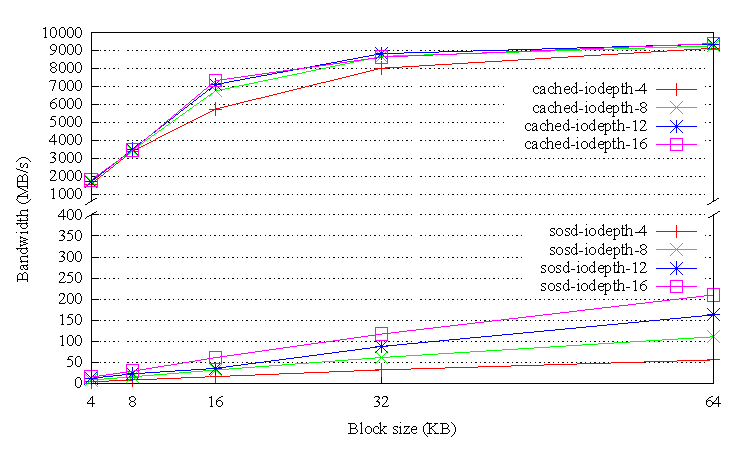
\includegraphics[width=\columnwidth]{images/bw-write-comp-lie.pdf}
			}
			Constants:
			\begin{itemize}
				\item cached has 4 threads
				\item workload size less than cache size
			\end{itemize}
		\end{column}
		\begin{column}{.5\textwidth}
			Read bandwidth
			\makebox[\textwidth]{
				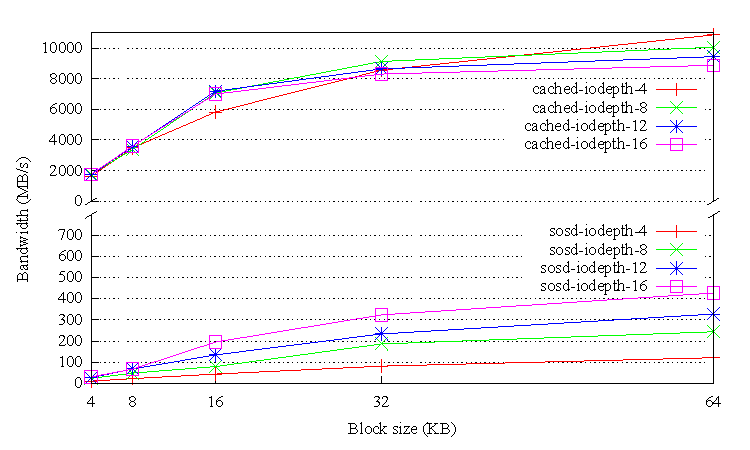
\includegraphics[width=\columnwidth]{images/bw-read-comp-lie.pdf}
			}
			Variables:
			\begin{itemize}
				\item block size [4KB - 64KB]
				\item parallel requests [4 - 16]
			\end{itemize}
		\end{column}
	\end{columns}

	\note[item]{Ας περιγράψουμε το benchmark μας. Στείλαμε καρφωτά στους peers 
		requests των...}
	\note[item]{Το iodepth είναι ο αριθμός των παράλληλων requests}
	\note[item]{Σημεία προσοχής:Για μικρά writes είμαστε έως 100x 
		γρηγορότεροι ενώ για μεγάλα έως 200x. }
	\note[item]{O cached μετά τα 16ΚΒ δεν κάνει scale - χτυπάμε το 
		bandwidth της RAM}
	\note[item]{Έχουμε lock contention, δε θα έπρεπε να αυξάνεται η 
		ταχύτητα για μεγάλα blocks και δεν αυξάνεται η ταχύτητα με 
		parallel requests}
	\note[item]{Lock contention είναι ότι δεν κάνουμε scale με πολλά threads 
		για μικρά block sizes}
\end{frame}

\begin{frame}{Cached/sosd comparison - peak behavior}
	\begin{columns}[t]
		\begin{column}{.5\textwidth}
			Write latency
			\makebox[\textwidth]{
				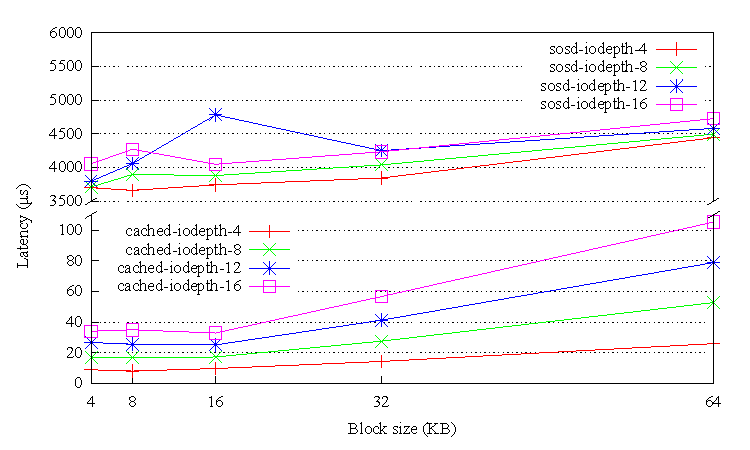
\includegraphics[width=\columnwidth]{images/lat-write-comp-lie.pdf}
			}
			Constants:
			\begin{itemize}
				\item cached has 4 threads
				\item workload size less than cache size
			\end{itemize}
		\end{column}
		\begin{column}{.5\textwidth}
			Read latency
			\makebox[\textwidth]{
				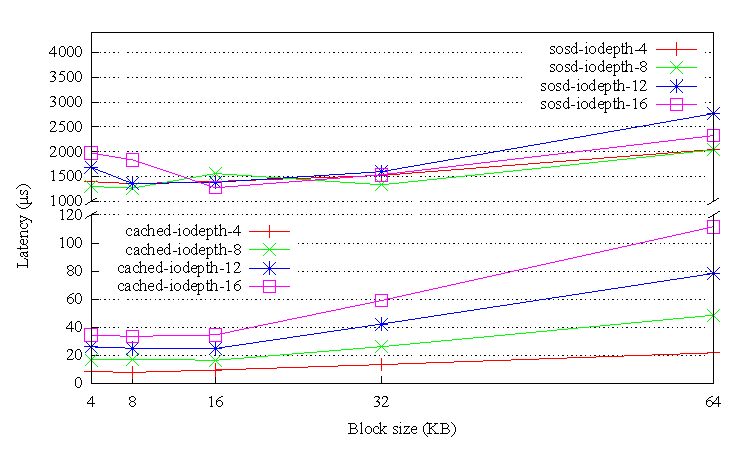
\includegraphics[width=\columnwidth]{images/lat-read-comp-lie.pdf}
			}
			Variables:
			\begin{itemize}
				\item block size [4KB - 64KB]
				\item parallel requests [4 - 16]
			\end{itemize}
		\end{column}
	\end{columns}

	\note[item]{Αντίστοιχα, για μικρά reads είμαστε 50x γρηγορότεροι ενώ 
		για μεγάλα έως 75x}
\end{frame}

\begin{frame}{Cached/sosd comparison - sustained behavior}
	\begin{columns}[t]
		\begin{column}{.5\textwidth}
			Write bandwidth
			\makebox[\textwidth]{
				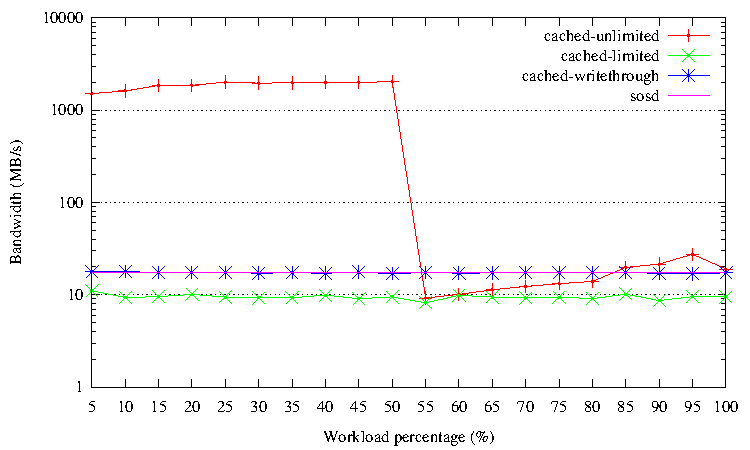
\includegraphics[width=\columnwidth]{images/bw-write-comp-truth.pdf}
			}
			Constants:
			\begin{itemize}
				\item cached has 4 threads
				\item workload twice the cache size
				\item block size is 4KB
				\item Parallel requests are 16
			\end{itemize}
		\end{column}
		\begin{column}{.5\textwidth}
			Write latency
			\makebox[\textwidth]{
				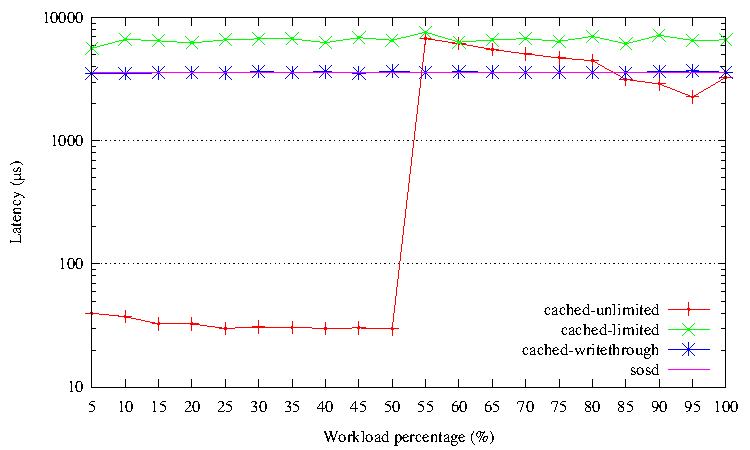
\includegraphics[width=\columnwidth]{images/lat-write-comp-truth.pdf}
			}
			Variables:
			\begin{itemize}
				\item cache write policy
				\item maximum cached objects
			\end{itemize}
		\end{column}
	\end{columns}

	\note[item]{unlimited: έχουμε περισσότερα buckets απ' ότι objects}
	\note[item]{Σημεία προσοχής: Writethrough όσο και το Rados ενώ στα 
		reads έχουμε παρατηρήσει καλύτερη ταχύτητα}
	\note[item]{Το performance πέφτει λόγω έλλειψης buckets, μεγαλώνει λόγω 
		coalesces}

\end{frame}

\begin{frame}{Cached internals - indexing}
	Latency of cold cache vs. warm cache
	\makebox[\textwidth]{
		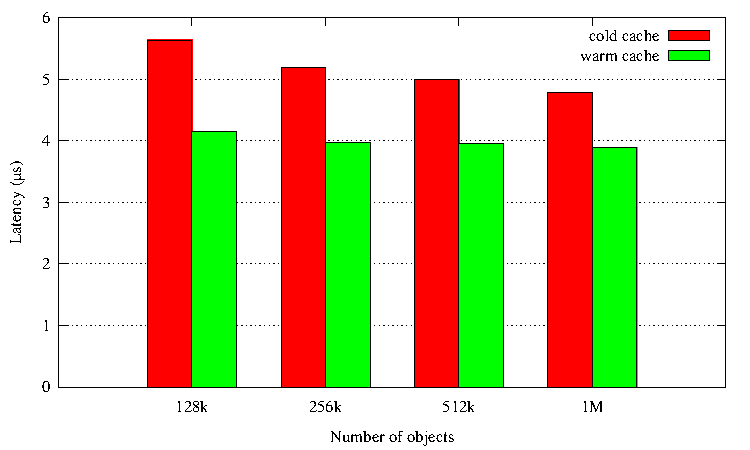
\includegraphics[width=0.45\textwidth]{images/cold1.pdf}
	}
	\begin{columns}[t]
		\begin{column}{.5\textwidth}
			Constants:
			\begin{itemize}
				\item workload less than the cache size
				\item block size is 4KB
				\item no threads or parallel requests 
			\end{itemize}
		\end{column}
		\begin{column}{.5\textwidth}
			Variables:
			\begin{itemize}
				\item number of objects [128k - 1M]
			\end{itemize}
		\end{column}
	\end{columns}
	\note[item]{Το σενάριο είναι το εξής. Εισάγουμε ένα αριθμό από objects.  
		Κάνουν lookup και insert. Μετά, τα κάνουμε lookup. Αυτό το κάνουμε για 
		128κ ... Μετράμε latency}
	\note[item]{Σταθερό indexing overhead. Αν πέσει ερώτηση πες 2Μ hash 
		table, το λειτουργικό δε δίνει αμέσως μνήμη}
\end{frame}

\begin{frame}{VM/Archipelago evaluation}
	\begin{columns}[t]
		\begin{column}{.5\textwidth}
			Write bandwidth
			\makebox[\textwidth]{
				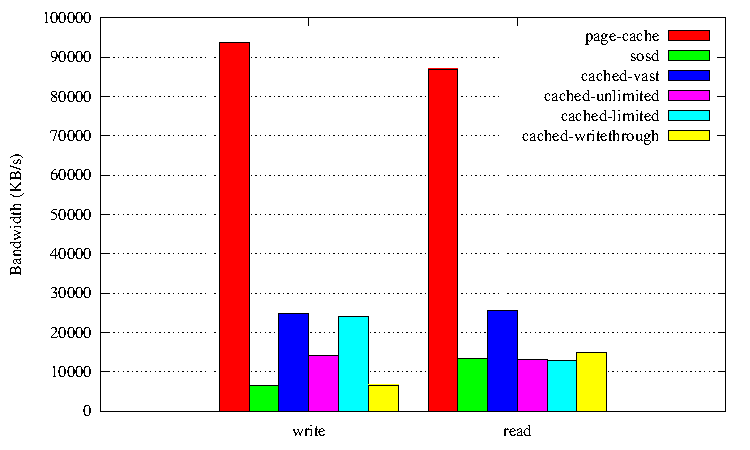
\includegraphics[width=\columnwidth]{images/bw-vm.pdf}
			}
			Constants:
			\begin{itemize}
				\item block size is 4KB
				\item parallel requests are 16
				\item cached has 4 threads
			\end{itemize}
		\end{column}
		\begin{column}{.5\textwidth}
			Write latency
			\makebox[\textwidth]{
				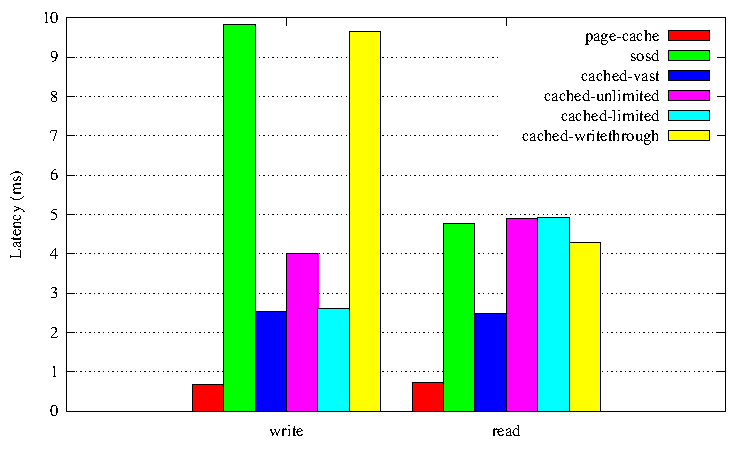
\includegraphics[width=\columnwidth]{images/lat-vm.pdf}
			}
			Variables:
			\begin{itemize}
				\item cache write policy
				\item maximum cached objects
			\end{itemize}
		\end{column}
	\end{columns}
	\note{Benchmark μέσα από το VM, με filesystem, elevators, κτλ. με το fio}
	\note{Σημεία προσοχής:
		\begin{itemize}
			\item page-cache: πολύ γρήγορη. Το 1ms latency λογικά 
				μπαίνει λόγω του paravirtualized storage, 
				filesystem, elevators
			\item sosd: είναι σίγουρα άσχημο αλλά σε αυτά τα test 
				έχει συν 7ms latency για τα writes και 3ms 
				latency για τα reads. Αυτό έιναι πολύ 
				μεγαλύτερο του 1ms του VM άρα κάτι παίζει με 
				Αρχιπέλαγο
			\item cached-vast: 4x γρηγορότερη από sosd αλλά έχει 
				3ms latency που δεν είχε πριν, δηλαδή το 
				archipelago βάζει 2ms
			\item cached-unlimited: 2.5x γρηγορότερο και ξεπέρασε 
				πάλι τον sosd στο τέλος
			\item cached-limited: 4x γρηγορότερο, λογικά τα flushes 
				είναι πολλα και μικρά και κρύβονται πίσω από το 
				latency του Archipelago
			\item writethrough δεν είδαμε κάποια διαφορά
		\end{itemize}
	}
\end{frame}





\section{Synapsed design}

\begin{frame}{Introduction}
	Previous results show that:
	\begin{itemize}
		\item There is high lock contention
		\item The amount of RAM is important
	\end{itemize}
	\note[item]{Από τα προηγούμενα συμπεράσματα, μπορούμε να εξάγουμε ότι 
		έχουμε τα εξής limitations ανεξαρτήτως latency Αρχιπελάγους: 
		lock contention και έλλειψη από RAM}
	\dspc
	If cached remains at the host, it will:
	\begin{itemize}
		\item Compete for CPU time
		\item Use a fraction of the host's RAM
	\end{itemize}
	\note[item]{Αν ο cached τρέχει στον host όπου τρέχουν και τα VMs, θα 
		έχουμε λιγότερη cpu -> περισσότερο contention και λιγότερη ram}
	\dspc
	Idea: what if cached ran on storage nodes?
	\note[item]{Αν έτρεχε στους αποθηκευτικούς κόμβους;}
\end{frame}

\begin{frame}
	If cached was on storage nodes, the pros would be:
	\begin{itemize}
		\item Access to more RAM
		\item Major step towards a distributed cache
	\end{itemize}
	\note[item]{Αν έτρεχε εκεί θα \todo}
	\dspc
	On the other hand, the cons would be:
	\begin{itemize}
		\item Network bottleneck
		\item Bigger complexity
	\end{itemize}
	\dspc
	Archipelago is network-unaware. Must create a proof-of-concept network peer 
	to help us in this task.
\end{frame}

\begin{frame}{Synapsed design}
	Synapsed is designed to do the following:
	\begin{itemize}
		\item Connect two Archipelago peers over network
		\item Forward read/write XSEG requests
		\item Use the TCP protocol
		\item Use vectored I/O, no intermediate copy
	\end{itemize}
	\dspc
	Replication should be trivial to implement, but it is currently missing.

	\note[item]{Το synapsed σχεδιάστηκε για τα εξής:
		\begin{itemize}
			\item Σύνδεση δυο Αρχιπέλαγο peers πάνω από network
			\item Κατάλληλη προώθηση I/O αιτημάτων
			\item Χρήση του tcp πρωτοκόλλου
			\item Χρήση μεθόδων διανυσματικού I/O χωρίς περιττά allocation 
				μνήμης
		\end{itemize}
	}
	\note[item]{H δημιουργία αντιγράφων μπορεί να προστεθεί εύκολα στα 
		παραπάνω, αλλά εμείς δεν φτάσαμε ώς εκει}

\end{frame}


\section{Synapsed evaluation}

\begin{frame}{Benchmark preamble}
	The most important part is that synapsed works. We are \textbf{now} able to
	run cached or part of Archipelago in the storage nodes.
	\dspc
	However, let's check its performance.
	\spc
	We will attempt to run most of the previous scenarios using synapsed this 
	time.
	\dspc
	Note, synapsed is proof-of-concept and not performance-tuned. Also, the 
	tested configuration uses a 1Gbit/s connection.
	\note[item]{O κύριως στόχος του synapsed είναι να προσφέρει τη 
		δυνατότητα ή ελαστικότηατα αν το θέλετε, του να τρέχει ο cached 
		ή κομματι του Archipelago σε άλλο κόμβο. Ας δούμε όμως την 
		επίδοσή του
	}
\end{frame}

\begin{frame}{Synapsed results}
	\begin{columns}[t]
		\begin{column}{.5\textwidth}
			Write bandwidth
			\makebox[\textwidth]{
				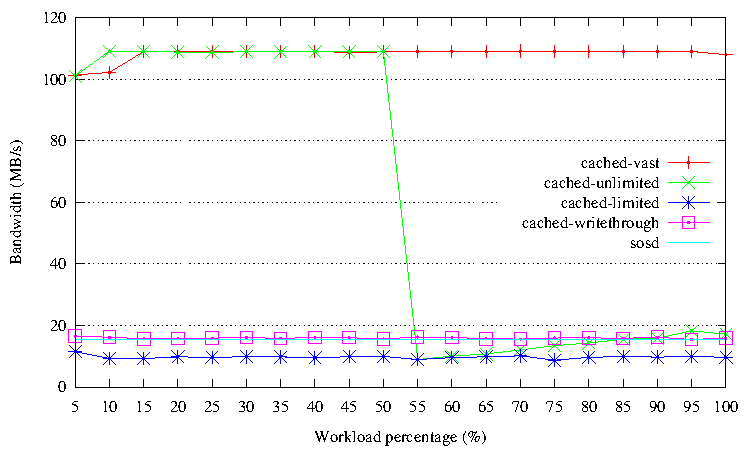
\includegraphics[width=\columnwidth]{images/bw-write-synapsed.pdf}
			}
			Constants:
			\begin{itemize}
				\item cached has 4 threads
				\item workload twice the cache size
				\item block size is 4KB
				\item Parallel requests are 16
			\end{itemize}
		\end{column}
		\begin{column}{.5\textwidth}
			Write latency
			\makebox[\textwidth]{
				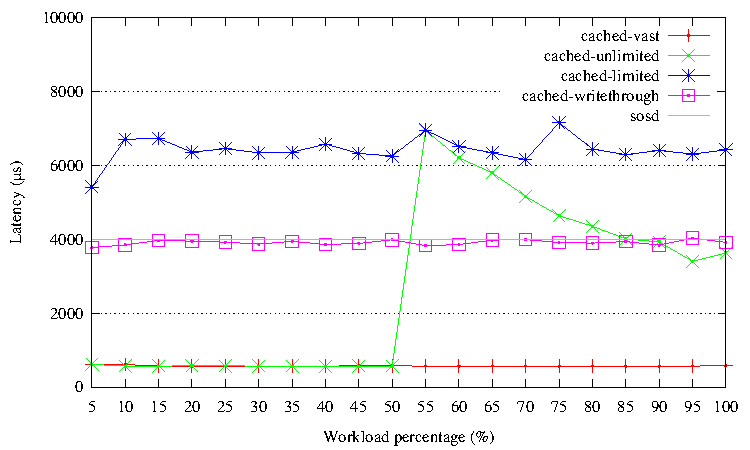
\includegraphics[width=\columnwidth]{images/lat-write-synapsed.pdf}
			}
			Variables:
			\begin{itemize}
				\item cache write policy
				\item maximum cached objects
			\end{itemize}
		\end{column}
	\end{columns}
	\note{Σημεία προσοχής, πρακτικά υπάρχει πολύ μικρή διαφορά με το διάγραμα 
		της σελίδας 32, απλά είναι CAPPED από το δίκτυο. Απλά μπάινει μικρότερο 
		του 1ms latency που για το cached-vast φυσικά κάνει μεγάλη 
		διαφορά.\dspc
		Κατά τα άλλα, το latency αυτό είναι αμελητέο σε σχέση με το 
		τρέχων latency, ενώ αν υπήρχε 10 ή 40Gbit δίκτυο, θα ήταν ακόμα 
		καλύτερα τα πράγματα.
	}
\end{frame}


\section{Conclusion}

\begin{frame}{Concluding remarks}
	We close this presentation with the following remarks:
	\begin{itemize}
		\item Cached and synapsed have covered important Archipelago needs
		\item Synthetic benchmarks show that cached can achieve 200x better 
			performance than sosd
		\item In more real-life scenarios, cached speeds Archipelago up to 
			400\%
		\item Synapsed can bridge two peers over network with minimal latency
	\end{itemize}
\end{frame}

\begin{frame}{Future work}
	Future work is happening as we speak:
	\begin{itemize}
		\item Full CoW support
		\item Namespace support
		\item Support for different policies and limits per volume
	\end{itemize}
\end{frame}

\begin{frame}{That's all folks!}

	\centering{\LARGE Questions?}

\end{frame}

\end{document}

